% begin module area-between-curves-intro
\begin{frame}
\frametitle{More About Areas}
Suppose two curves, $y = f(x)$ and $y = g(x)$, are given.

How do we find the area bounded by those curves between the endpoints $x = a$ and $x = b$?

%\begin{center}
\hfil\hfil\psset{xunit=1cm, yunit=1cm}
\begin{pspicture}(-0.5, -0.5)(4.2,3.7)
\psframe*[linecolor=white](-0.5, -0.5)(4.2,3.7)
\tiny
\psaxes[ticks=none, labels=none]{<->}(0,0)(-0.5,-0.5)(4,3.5)
\fcLabels{4}{3.5}
\fcXTickWithLabel{0.5}{$a$}
\fcXTickWithLabel{3}{$b$}
\rput[bl](3.1, 3){$y=f(x)$}
\rput[l](3.1, 1.3){$y=g(x)$}
\pscustom*[linecolor=\fcColorAreaUnderGraph]{
%Function formula: (1/4 (x))^{2}+2
\psplot[plotpoints=1000]{0.5}{3}{2 x 0.25 mul 2 exp add }
%Function formula: 3/2- ((-3/4+1/4 (x))^{2})
\psplot[plotpoints=1000]{3}{0.5}{x 0.25 mul -0.75 add 2 exp -1 mul 1.5 add }
}
%Function formula: (1/4 (x))^{2}+2
\psplot[linecolor=\fcColorGraph, plotpoints=1000]{0}{4}{2 x 0.25 mul 2 exp add }
%Function formula: 3/2- ((-3/4+1/4 (x))^{2})
\psplot[linecolor=\fcColorGraph, plotpoints=1000]{0}{4}{x 0.25 mul -0.75 add 2 exp -1 mul 1.5 add }
\end{pspicture}
%\end{center}
%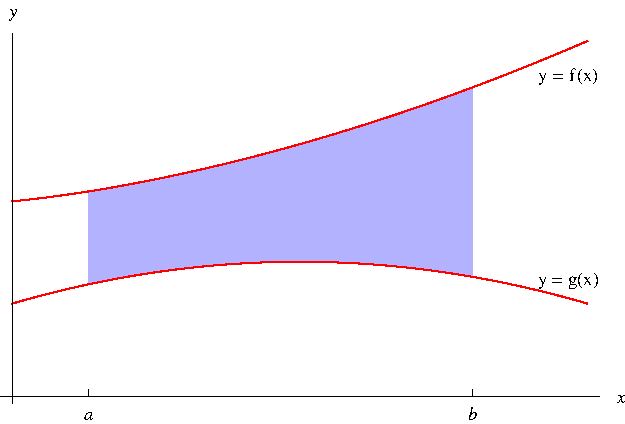
\includegraphics[height=3cm]{area-between-curves/pictures/06-01-doubleint.pdf}
\end{frame}
% end module area-between-curves-intro
